\documentclass[oneside]{book}

\usepackage{../pyhelp} 
 
\setcounter{chapter}{-1} 
    
    \title{Python Guide\\Chapter 0 - Installation and Workflow}
    
    \author{Daniel Scarbrough}
    \date{\today}
    
\makeindex

\begin{document}
\maketitle

\tableofcontents

\chapter{Installation and Workflow}
This chapter is a brief getting started guide to get Python installed and running on your machine. Beyond installation, there are also many different "workflows" you can adopt. This is just how you choose to edit and run your code, and this is up entirely to your personal preference. So try something and if it doesn't feel right, try another! Please reach out with any installation difficulties to dscarbro@mines.edu

\section{Installation Option 1 - "Classic"}
The first step is to get Python installed on your computer. Check the following subsections for your operating system for a guide.

\subsection{Windows 10}
Getting Python going on Windows is relatively easy but there are a few tricks to watch out for, so read carefully! 

First, go to the Python official website at \url{https://www.python.org/downloads}. At the time of writing (February 2021), there is a Python Version 3.9 available. This version is pretty new and not all commonly used packages for what we need are officially supported in 3.9. For this reason, \textbf{we want to install version 3.8} (current package support can be found at \url{https://pyreadiness.org}).

\begin{figure}[H]
\centering
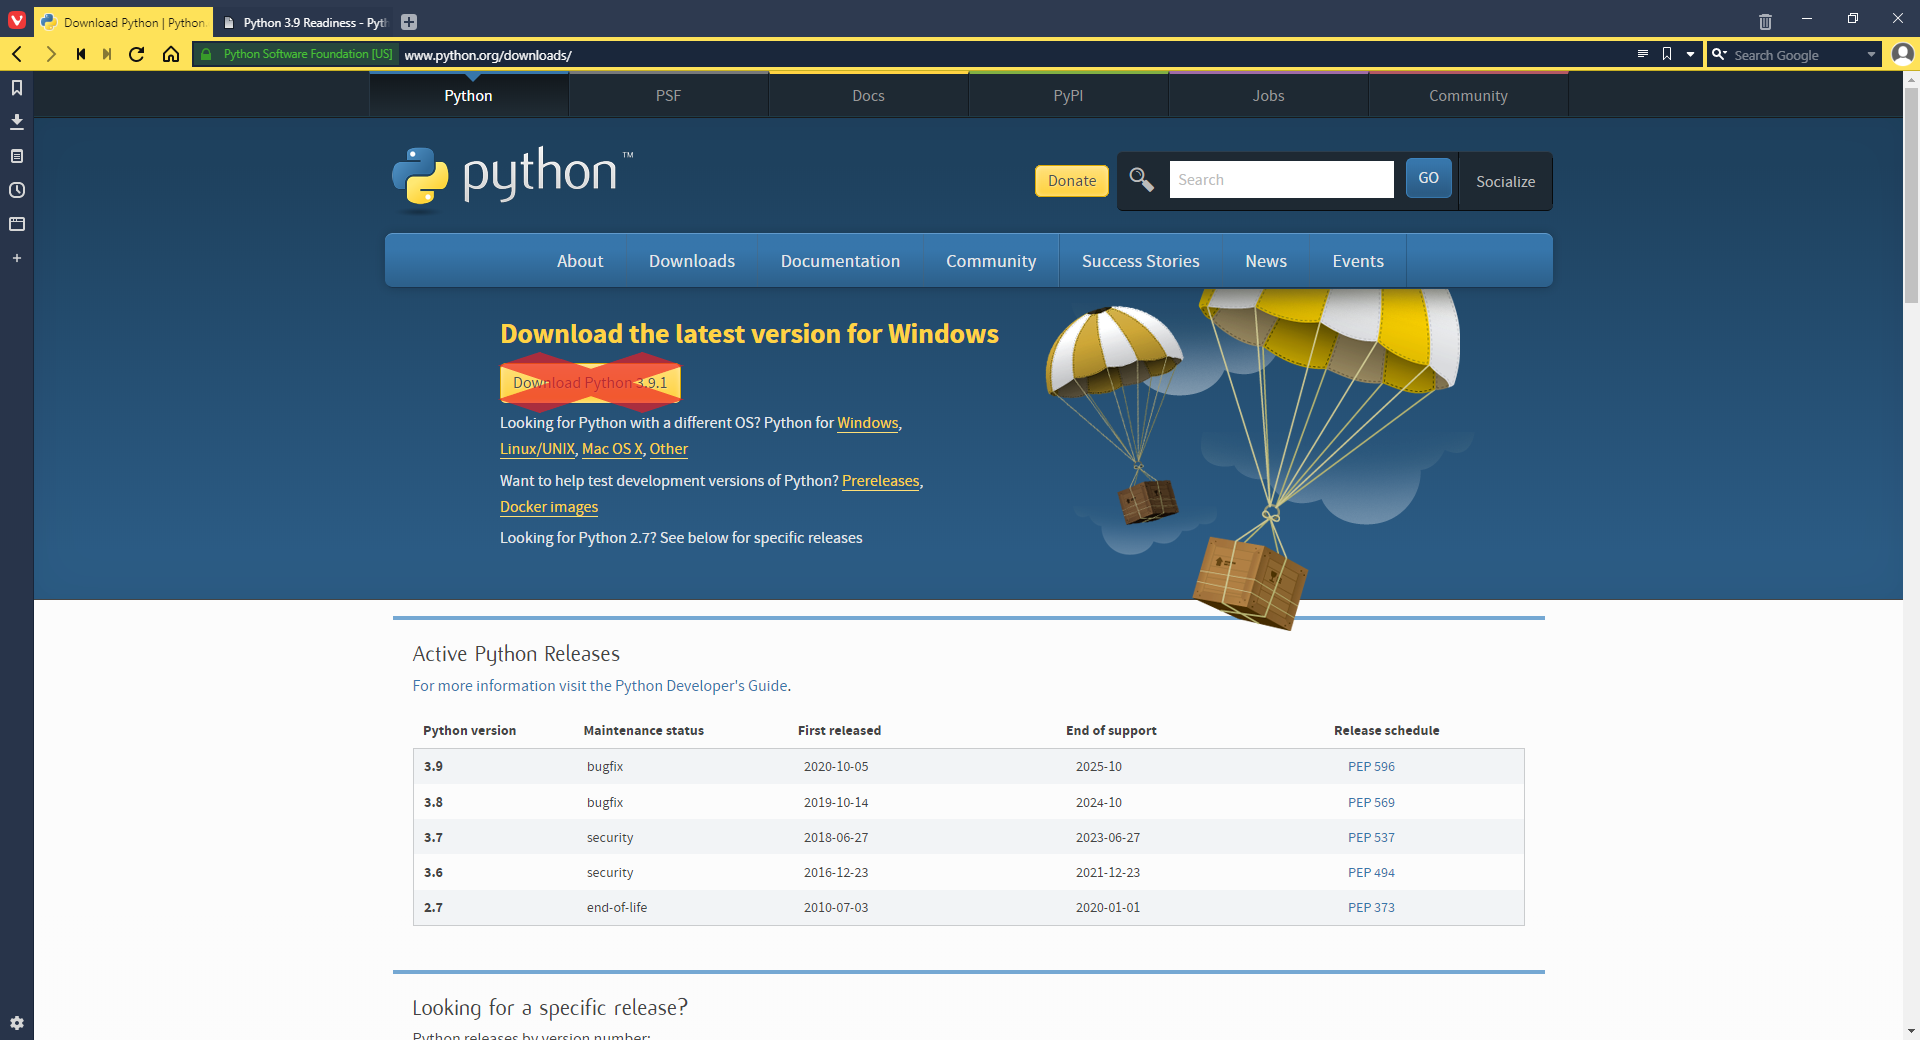
\includegraphics[width=0.7\linewidth]{./img/pyDownloadStart.PNG}
\caption{The Python downloads page. Don't click on the shiny big button (Feb. 2021) - the newest version may not have official support from all major packages for a few months or more from its initial release.}
\label{fig:pyhomepage}
\end{figure}

\FloatBarrier

Instead of the shiny big button, scroll down to see the latest releases for each version. In February 2021, the most recent version with support from most major packages is 3.8.7 - as seen in Figure \ref{fig:pyDownloadVersions}. Click the associated download link to continue.

\begin{figure}[H]
\centering
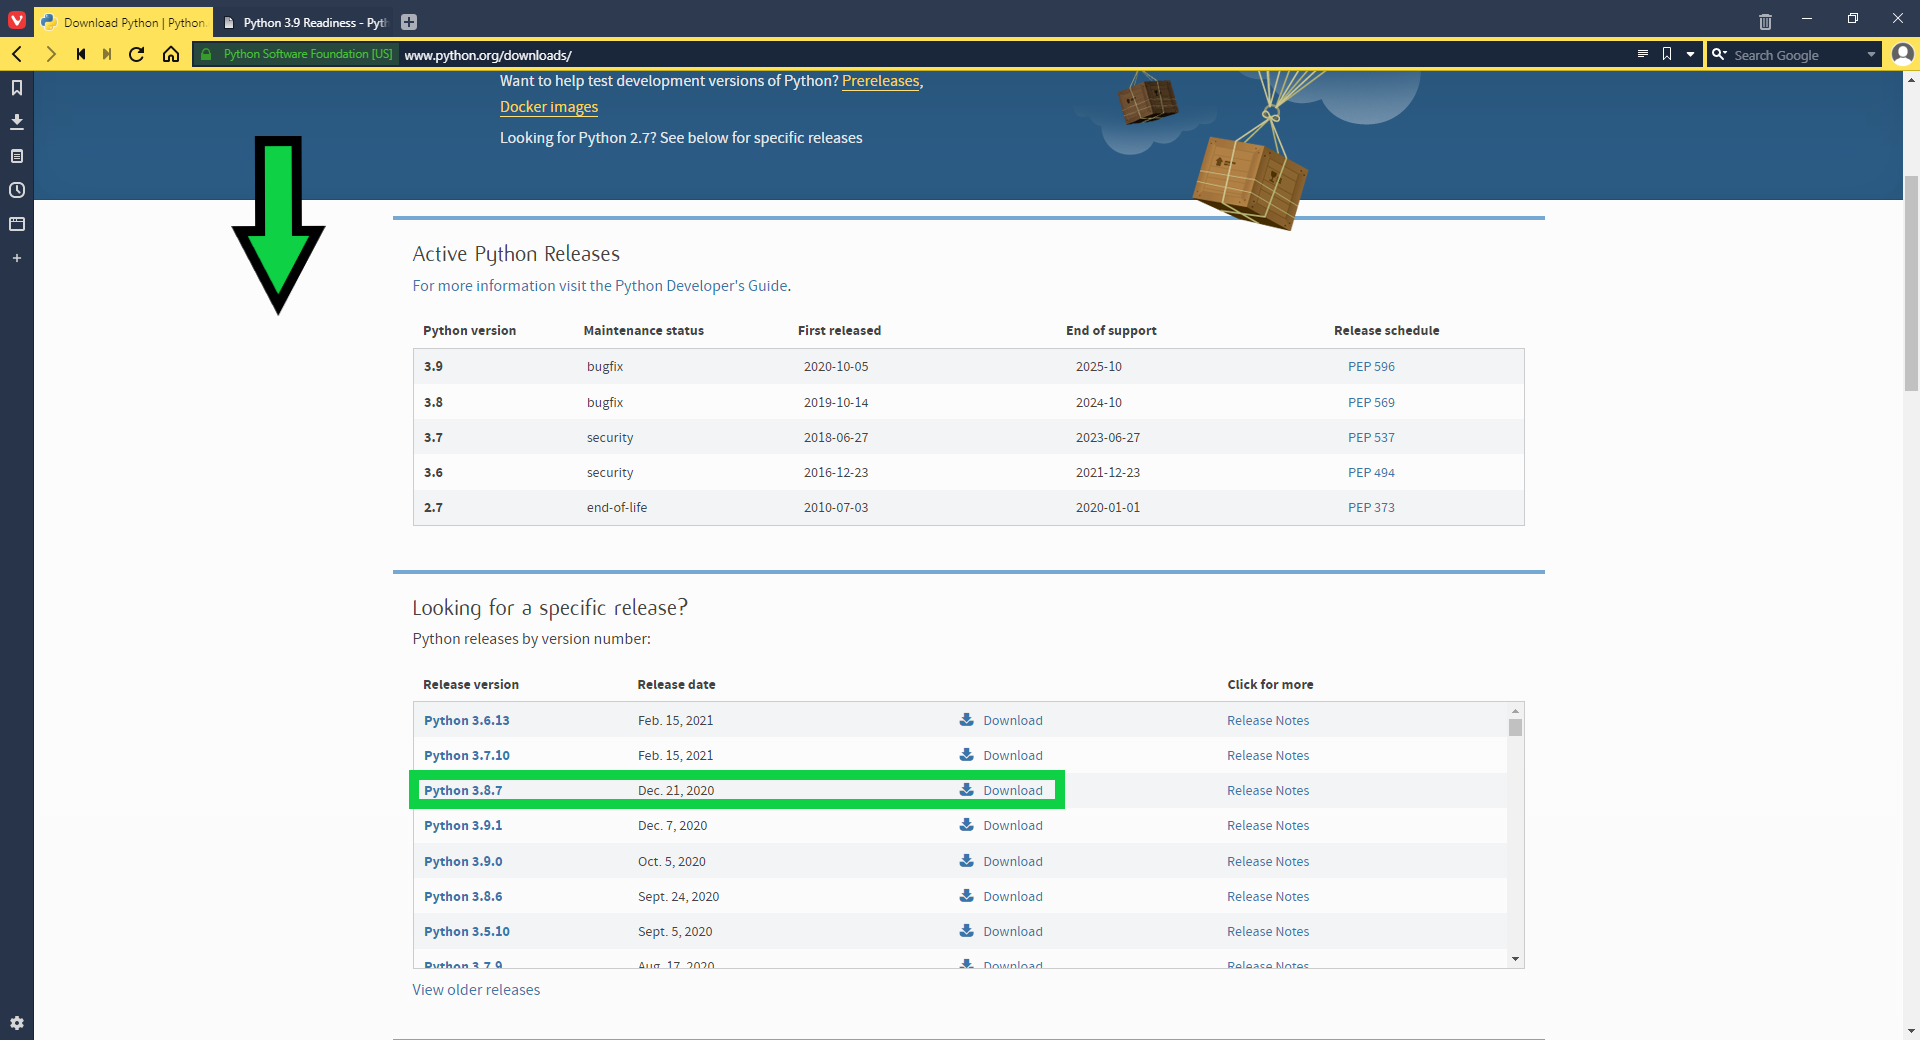
\includegraphics[width=0.7\linewidth]{./img/pyDownloadVersion.PNG}
\caption{Latest version releases of Python. At this time we are looking for the latest 3.8.x version.}
\label{fig:pyDownloadVersions}
\end{figure}

\FloatBarrier

Now that we are looking at the right version, we can go ahead and download the easy-to-use installer. Scroll down and look for the Windows Installers (boxed in Figure \ref{fig:pyInstallSelect}). It is important you choose the right installer for either a 32-bit or 64-bit system. If you are unsure, right-click on your Windows start menu icon and select "System". Under "Device Specifications" and "System Type" you will see either \textbf{64-bit operating system, x64-based processor} or \textbf{32-bit operating system, x86-based processor}. Select the correct installer link and go ahead and run the \texttt{.exe} file, but pause before clicking through the installer!

\begin{figure}[H]
\centering
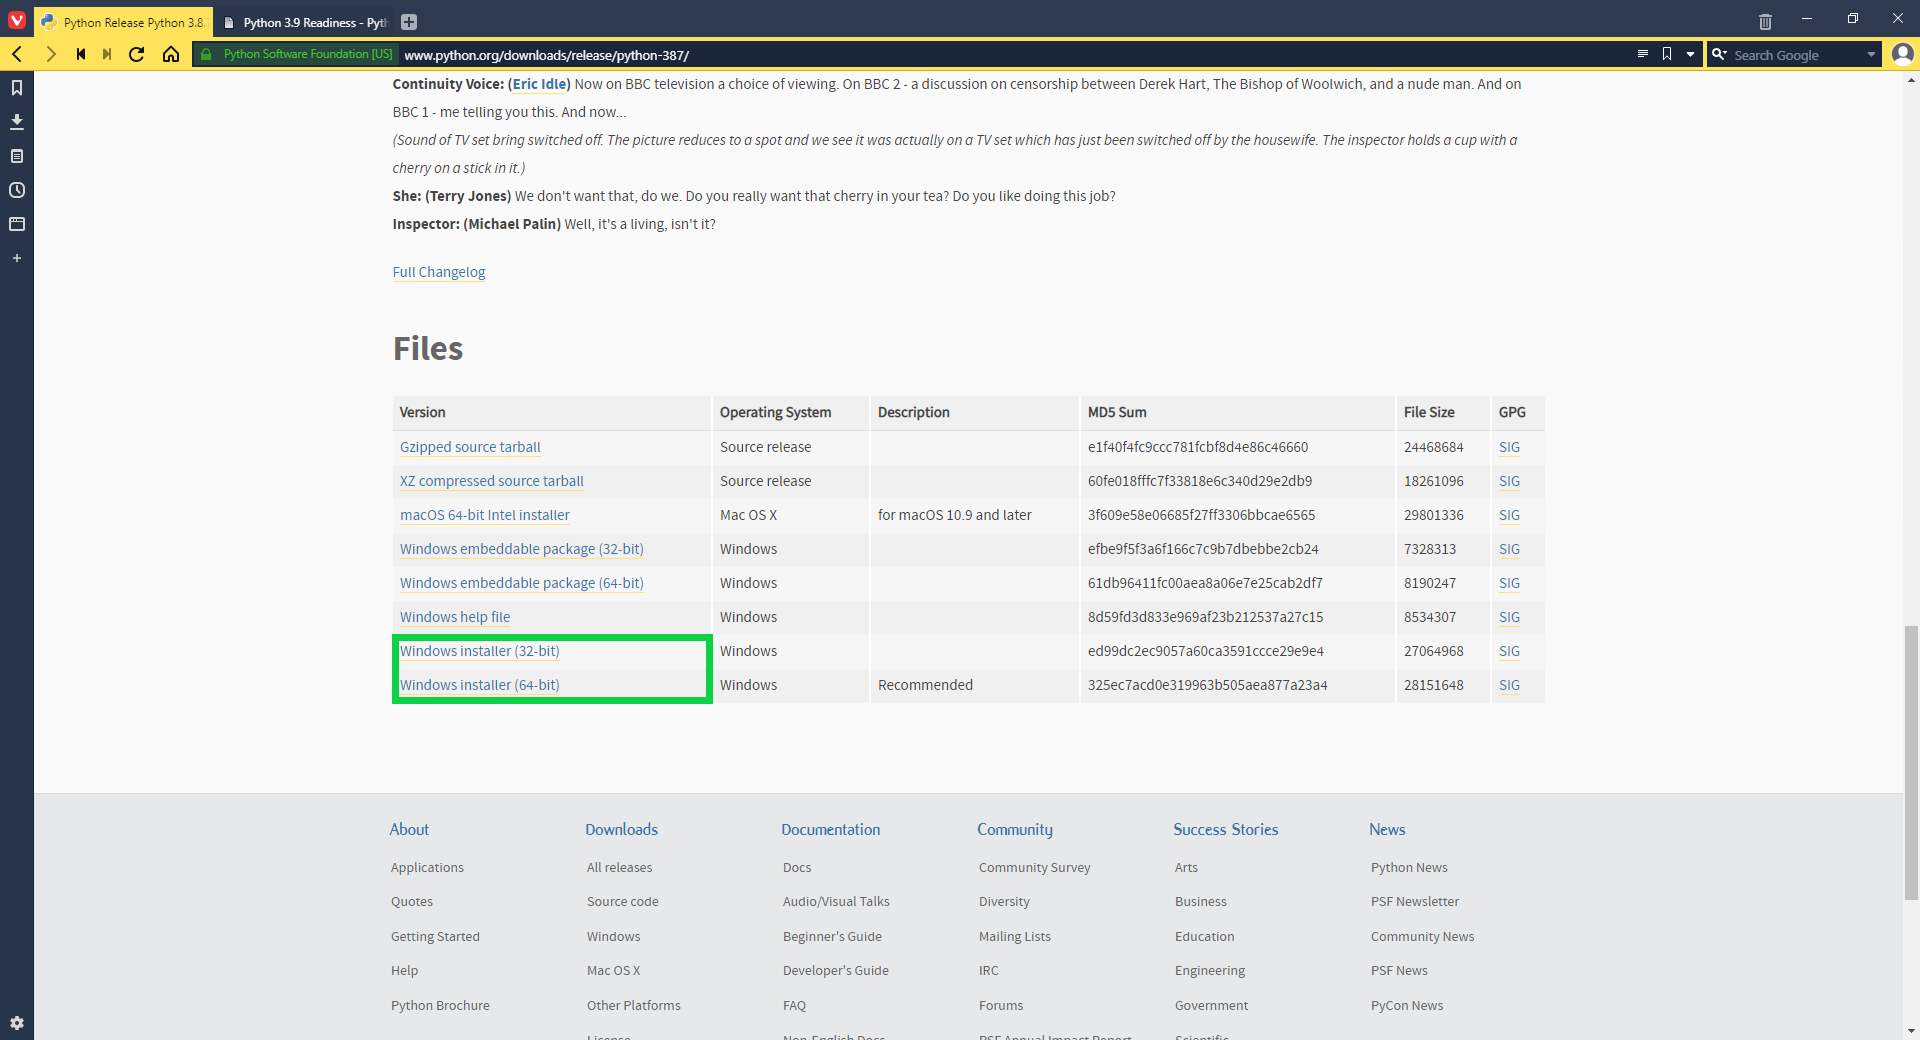
\includegraphics[width=0.7\linewidth]{./img/pyDownloadOS.PNG}
\caption{Select the installer for Windows, but be careful to select the correct processor type.}
\label{fig:pyInstallSelect}
\end{figure}

Once the installer is downloaded, go ahead and run it (will automatically run if you selected "open" when downloading). \textbf{Pause} here - you need to check the box to add Python to PATH. Otherwise, Windows won't know where to look when you ask it to use Python. Once that box is checked go ahead with the installation.

\begin{figure}[H]
\centering
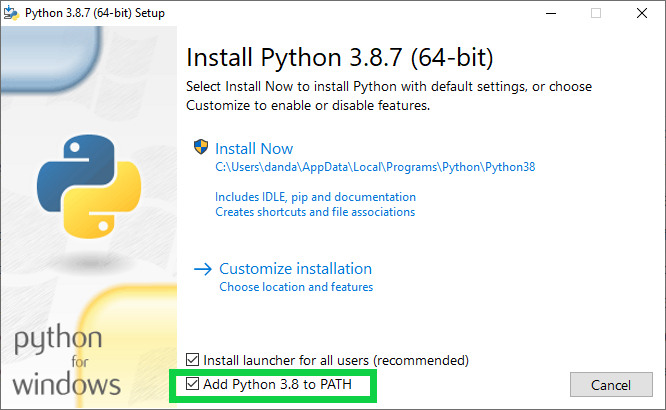
\includegraphics[width=0.7\linewidth]{./img/pyInstaller.PNG}
\caption{Checking the box to add Python to the system PATH so Windows can always find it.}
\label{fig:pyInstaller}
\end{figure}

\subsection{Linux}

There's a really good chance Python is already on your Linux system. One thing to be careful of is that sometimes this includes Python 2.x and Python 3.x! You can check by typing \texttt{python --version}. If it spits back a 2.x version, try \texttt{python3 --version}. If it isn't there at all, install it with your distro's package manager. Note that if you have both Python 2 and Python 3, you will have to be careful when installing packages: \texttt{pip} and \texttt{pip3} will install packages for each separately.

\subsection{Mac OS}

Work in progress

\subsection{Testing the Installation and Installing Packages}

To check that everything is working we can run Python directly from a terminal. The following images show how to do so on Windows, but the instructions are the same for pretty much any terminal.

On Windows, we will use the PowerShell rather than the Command Line. PowerShell uses most of the same commands you would see on a Linux system so it is great practice. To start, search PowerShell in your start menu (I recommend pinning it to the start menu or taskbar if you'll be using it a lot). 

\begin{figure}[H]
\centering
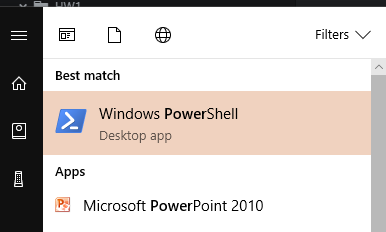
\includegraphics[width=0.5\linewidth]{./img/powershell.PNG}
\caption{Opening Windows PowerShell}
\label{fig:powershell}
\end{figure}

With your terminal open, go ahead and type \texttt{python --version}. If everything installed correctly, you should see a version return. If you get an error ensure your installation finished without error, and if on Windows, ensure that it got added to your path. Googling "Windows 10 check path" will get you what you need, but feel free to reach out with questions. Now, from a terminal if you just type \texttt{python} (or \texttt{python3} if on a machine with both version 2 and 3) and hit enter. You can now enter the mandatory first line:

\texttt{print("hello world!")}

It will just echo this back at you, but it's a necessary step. You can also start running various commands in here, including math. When you're done with Python in this terminal, you can enter \texttt{quit()} to stop running Python commands.

\begin{figure}[H]
\centering
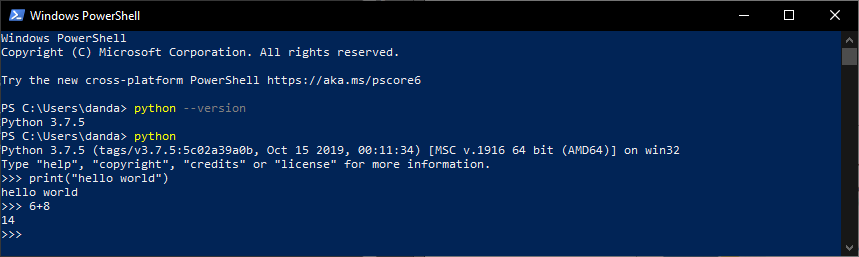
\includegraphics[width=0.7\linewidth]{./img/pythonTestRun.PNG}
\caption{Checking the Python version and running Python directly in the shell. On this system I am have an installation from before version 3.8.}
\label{fig:powershellTest}
\end{figure}

Now just to get Terminal navigation down if you're not familiar - here are four basic things to know:

\begin{itemize}
	\item{\makebox[2cm][l]{\texttt{cd} $<$dir$>$} "Change Directory" - moves the terminal to the location specified by \texttt{dir}.}
	\item{\makebox[2cm][l]{\texttt{ls}} "List Segment" - Show all files and folderss visible in current location}
	\item{\makebox[2cm][l]{\texttt{.}} "Current Directory" - single dot indicates that file paths start from current location.}
	\item{\makebox[2cm][l]{\texttt{..}} "Parent Directory" - two dots indicates the directory above the current directory.}
\end{itemize}

An example of each of these commands is shown in Figure \ref{fig:pytest}. In this example I have made a directory in my Documents directory called "pytest". And within that I have a Python file called \texttt{test.py}. 

\begin{figure}[H]
\centering
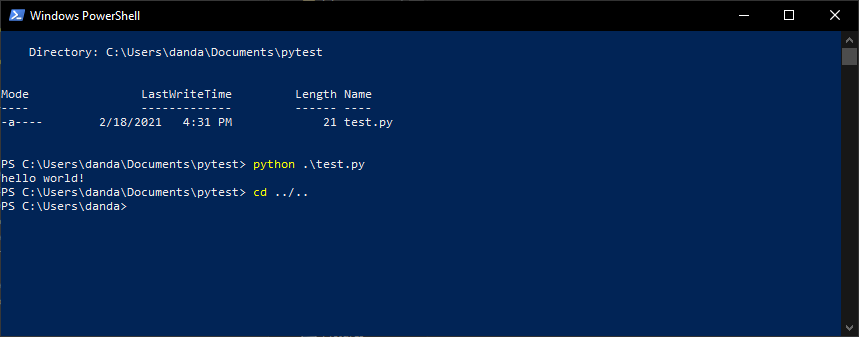
\includegraphics[width=0.7\linewidth]{./img/pytest.PNG}
\caption{Navigating directories in the terminal and running a python script. Take note of the \texttt{..} and \texttt{.} in the file paths. When using a terminal, tab will autocomplete file names which can be very handy!}
\label{fig:pytest}
\end{figure}

\subsubsection{Installing Packages}

Lastly, one important step. Python is open source and packages are developed by people of all backgrounds and fields. Base Python is pretty great, but to really make it worthwhile you'll want some packages. The best part is - they are all entirely free. As a brief side-note: this means that any work you do in Python and share with others both recreationally and for work/academics/etc. will be usable by anyone; no one will be shut out from collaborating and learning due to massive licensing fees!

Continuing on, pretty much all Python installations will include the package manager \texttt{pip}. If you're on Linux with both Python 2 and 3, make sure you work with \texttt{pip3} to install to the right version! For the first few chapters you will definitely need \texttt{numpy} and \texttt{matplotlib}. These are installed by entering:

\texttt{pip install numpy}\\
\texttt{pip install matplotlib}

You should see a confirmation message barring any errors. Now you are ready to decide how you want to code!

\section{Installation Option 2 - Anaconda}

Another route you can go is to use Anaconda to install and manage packages. This is documented well on their website here: \url{https://www.anaconda.com/products/individual}

I used Anaconda with the Spyder IDE many many years ago, so I cannot currently speak to its pros and cons over the "classic" installation and package management.

\section{Workflow}

There are a ton of options for how you can write and run your Python code. There is no "right answer", it's entirely up to your personal preference. You can pick a favorite text editor (not Word though, please!) and run code from the terminal, or you can use an Integrated Development Environment (IDE). The Spyder IDE is popular and feature-rich, and PyCharm is another popular option. Feel free to look in to them and see if they might work for you.

Personally, I prefer a rich text-editor with tons of useful extensions and customization. I've used a few, but for a few years now I've been using Visual Studio Code (VSCode, not to be confused with Visual Studio for C++ programming). Again if you go the text-editor + terminal route there is a lot to choose from. Some options are:

\begin{itemize}
\item If you want literally no features:
\begin{itemize}
\item Notepad
\end{itemize}
\item If you want to go old school with a robust terminal editor:
\begin{itemize}
\item Vim
\item eMacs
\end{itemize}
\item Customizable and extension-supporting editors:
\begin{itemize}
\item Notepad++
\item Atom
\item Sublime
\item VSCode
\end{itemize}
\end{itemize}

If you're completely unsure where to start, I will share part of my setup as an example. I have VSCode and the following extensions installed (ignoring non-applicable to Python extensions):

\begin{itemize}
\item Atom One Dark Theme - My favorite dark color theme
\item Python - Handles auto complete and error checking
\item Todo Tree - Highlights statements like "TODO" and "FIXME" + more
\item vscode-icons - Nicer looking icons
\item GitHub extensions (guides coming in the future)
\end{itemize}

I've also set up shortcuts and other convenient things in VSCode, plus some simple things like a line-ruler at 79 characters to keep it readable - but those things are not at all necessary until you decide you want it. Take some time to shop around - and if you try one thing and it doesn't vibe - try something else! Feel free to reach out with questions about editors, IDEs, making it look cool, macros, etc. Now to code!

\begin{figure}[H]
\centering
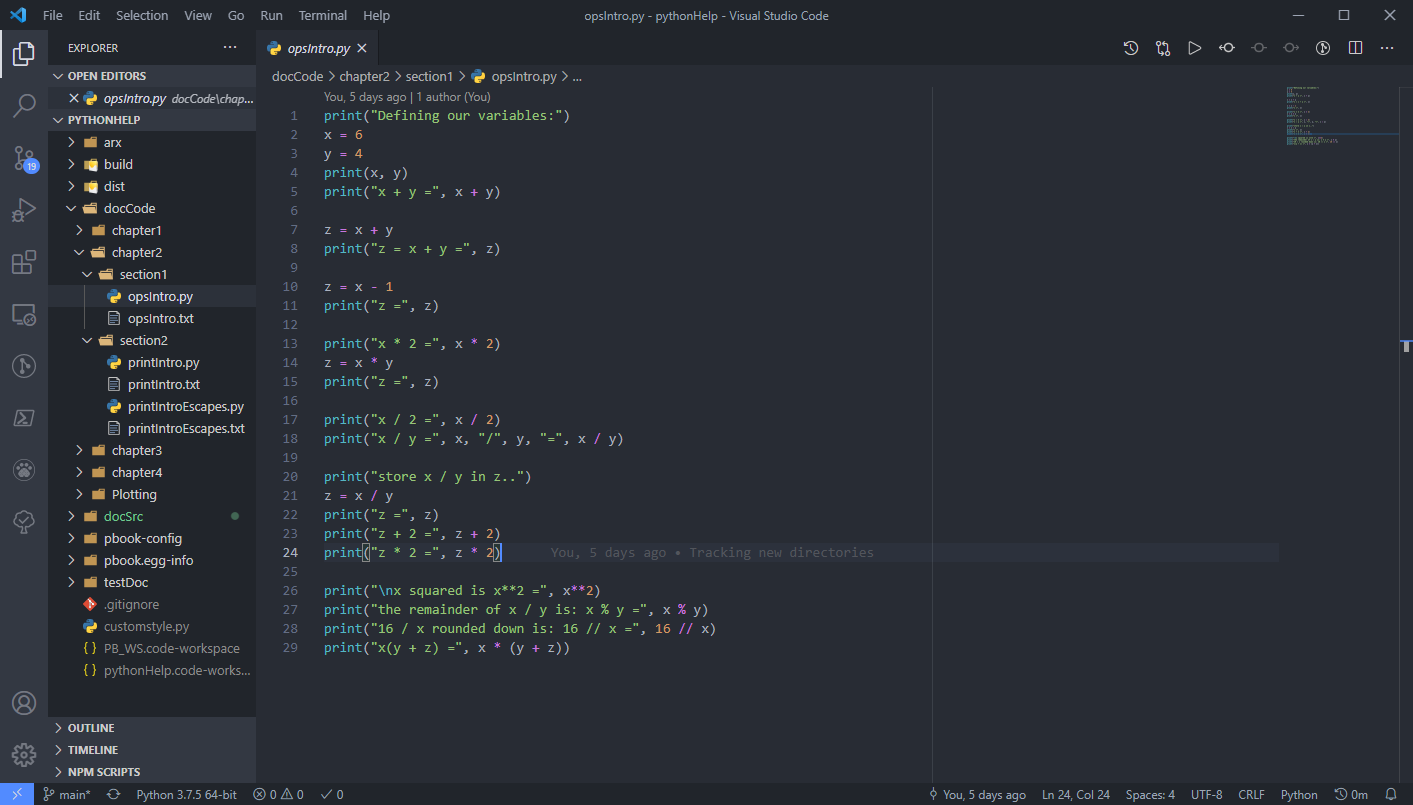
\includegraphics[width=0.8\linewidth]{./img/vscodeExample.PNG}
\caption{A screenshot of editing Python in VSCode}
\label{fig:vscode}
\end{figure}

\end{document}